% Copyright (c) 2012 by Michał Nazarewicz <mina86@mina86.com>
% Distributed under the terms of the Creative Commons
% Attribution-ShareAlike 3.0 Unported (CC BY-SA 3.0) license.

\subsection{Page allocator}

\begin{frame}[fragile]
  \frametitle{Linux kernel memory allocators}

  \begin{center}
    \includegraphics<1>[width=\textwidth]{build/linux-allocators--base.eps}
    \includegraphics<2>[width=\textwidth]{build/linux-allocators--important.eps}
  \end{center}
\end{frame}

\begin{frame}
  \frametitle{Buddy allocator}
  \begin{columns}[c]

    \column{0.6\textwidth}
    \begin{itemize}
    \item Page allocator uses buddy allocation algorithm.
      \begin{itemize}
      \item Hence different names: buddy system or buddy allocator.
      \end{itemize}
    \item Allocations are done in terms of orders.
    \item User can request order from 0 to 10.
    \item If best matching page is too large, it's recursively split
      in half (into two buddies).
    \item When releasing, page is merged with its buddy (if free).
    \end{itemize}

    \column{0.4\textwidth}
    \begin{center}
    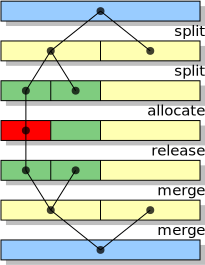
\includegraphics[width=0.9\textwidth]{build/alloc-free-cycle.eps}
    \end{center}
  \end{columns}
\end{frame}

\begin{frame}
  \frametitle{Pages and page blocks}
  \begin{center}
  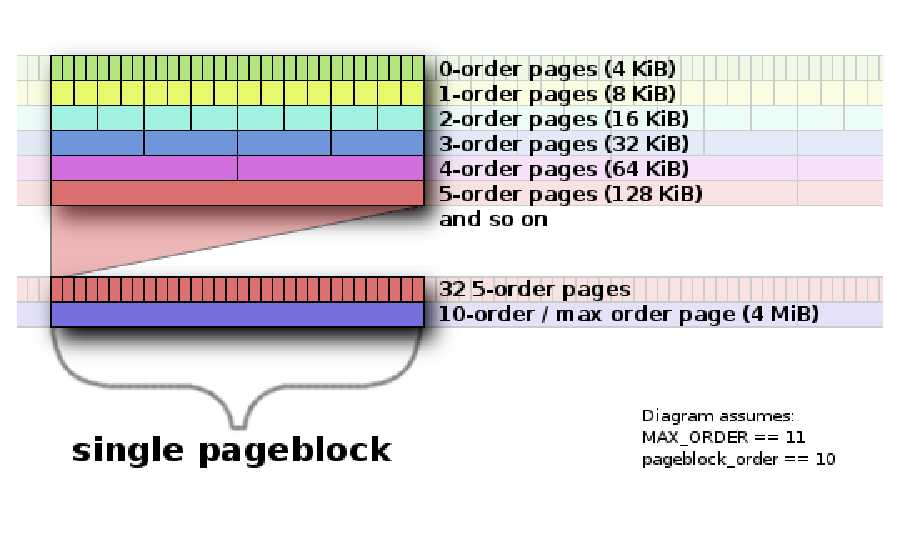
\includegraphics[width=0.9\textwidth]{build/pages.eps}
  \end{center}
\end{frame}

\begin{frame}[fragile]
  \frametitle{Migrate types}

  \begin{itemize}
  \item On allocation, user requests an unmovable, a~reclaimable or
    a~movable page.
    \begin{itemize}
    \item For our purposes, we treat reclaimable as unmovable.
    \end{itemize}
  \item To try keep pages of the same type together, each free page
    and each page block has a~migrate type assigned.
    \begin{itemize}
    \item But allocator will use fallback types.
    \item And migrate type of a~free page and page blocks can change.
    \end{itemize}
  \item When released, page takes migrate type of pageblock it belongs
    to.
  \end{itemize}
\end{frame}
